\chapterimage{chapter_head_1.pdf} 
\chapter{Realización de un juego con gráficos}

En este capítulo, se darán las instrucciones para la realización paso a paso de un videojuego usando el sistema gráfico de la NDS. La lista de ejercicios y el tiempo estimado (en minutos) para su realización se muestra en la Tabla \ref{c10_tab:ejercicios}.

\begin{table}[t]
	\centering
	\caption{Ejercicios del capítulo y tiempo estimado para su realización.}
	\begin{tabular}{|c|c||c|c|}
		\hline 
		Ejercicio & Tiempo & Ejercicio & Tiempo\\ 
		\hline 
		10.1 & 10' & 10.7  & 20'  \\ 
		10.2 & 20' & 10.8  & 40' \\ 
		10.3 & 30' & 10.9  & 20' \\ 
		10.4 & 20' & 10.10 & 40' \\ 
		10.5 & 20' & & \\
		10.6 & 20' & & \\ 
		\hline 
	\end{tabular} 
	\label{c10_tab:ejercicios}
\end{table}

% -------------------------------------------------------------------------
% -------------------------------------------------------------------------
% -------------------------------------------------------------------------
% -------------------------------------------------------------------------
\section{Descripción del juego}
El juego que se va a realizar es una versión simplificada del típico juego en el que una rana tiene que cruzar una carretera llena de vehículos evitando ser atropellada. La Figura \ref{fig:c7_frogs}\footnote{La imagen se ha obtenido en la siguiente web: \url{https://frogmatters.files.wordpress.com/2008/04/frogster.png}} muestra un ejemplo de este tipo de juego. En el siguiente vídeo \url{https://www.youtube.com/watch?v=OpuduHSWBcw} podemos ver el funcionamiento de una versión de este juego.

\begin{figure}[t]
	\centering
	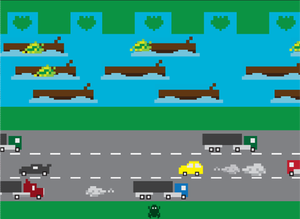
\includegraphics[height=7cm]{Figuras/C10/c10_frogs.png}
	\caption{Juego \textit{Crossing frogs}.}
	\label{fig:c7_frogs}
\end{figure}

En la versión que se va a desarrollar se usarán los conceptos aprendidos en los capítulos 5, 6, 7, 8 y 9. 

% -------------------------------------------------------------------------
% -------------------------------------------------------------------------
% -------------------------------------------------------------------------
% -------------------------------------------------------------------------
\section{Desarrollo del juego}
La parte gráfica del juego se visualizará en la pantalla inferior. En la pantalla superior se mostrarán mensajes sobre el juego. Se pondrán realizar más de una partida, puesto que el objetivo será llegar a la meta intentando superar el récord actual. Para todas las cuestiones relacionadas con la entrada y salida (botones y temporizadores) se deberán emplear interrupciones.

% -------------------------------------------------------------------------
% -------------------------------------------------------------------------
\subsection{Primeros pasos}
En primer lugar debemos crear las teselas para los gráficos del juego. Crearemos 6 teselas diferentes:
\begin{itemize}
	\item Tesela 0: La rana.
	\item Tesela 1: Filas inferiores que serán la de posición inicial de la rana.
	\item Tesela 2: Fila superior que es donde tiene que llegar la rana.
	\item Tesela 3: Fondo de la carretera.
	\item Tesela 4: Línea que divide la carretera.
	\item Tesela 5: Vehículo que hay que evitar.
\end{itemize}

\begin{example}
El programa \textit{ranas\_inicial.c} muestra un ejemplo de las 6 teselas creadas y colocadas en la pantalla. El programa principal del mismo es el siguiente (en el programa completo están definidas las teselas y el mapa de teselas):

\begin{lstlisting}
...
int main( void )
{
	int fila;
	int columna;
	int pos_mapMemory;
	int pos_mapData;
	int record;
	int tiempo;
	
	REG_POWERCNT = POWER_ALL_2D;
	REG_DISPCNT  = MODE_0_2D   | DISPLAY_BG0_ACTIVE ;
	VRAM_A_CR    = VRAM_ENABLE | VRAM_A_MAIN_BG ;
	BGCTRL [0]   = BG_32x32    | BG_COLOR_256 | BG_MAP_BASE(0) | BG_TILE_BASE(1);
	
	static u8*  tileMemory = (u8*)  BG_TILE_RAM(1);
	static u16* mapMemory  = (u16*) BG_MAP_RAM(0);
	
	BG_PALETTE[0]=RGB15( 0, 0, 0); // Negro
	BG_PALETTE[1]=RGB15(31,31,31); // Blanco
	BG_PALETTE[2]=RGB15(15,15,15); // Gris
	BG_PALETTE[3]=RGB15( 0,31, 0); // verde
	BG_PALETTE[4]=RGB15(20,20,0);  // amarillo apagado
	BG_PALETTE[5]=RGB15( 0, 0,31); // azul
	
	dmaCopy(t_rana,      tileMemory ,      sizeof(t_rana));
	dmaCopy(t_salida,    tileMemory + 64,  sizeof(t_salida));
	dmaCopy(t_meta,      tileMemory + 128, sizeof(t_meta));
	dmaCopy(t_carretera, tileMemory + 192, sizeof(t_carretera));
	dmaCopy(t_mitad,     tileMemory + 256, sizeof(t_mitad));
	dmaCopy(t_coche,     tileMemory + 320, sizeof(t_coche));
	
	pos_mapData = 0;
	for(fila=0;fila<24;fila++)
	  for(columna=0;columna<32;columna++)
      {
		pos_mapMemory            = fila*32+columna;
		mapMemory[pos_mapMemory] = mapData[pos_mapData];
		pos_mapData ++;
	  }
	
	consoleDemoInit();
	
	tiempo = 0;
	record = 1000;
	while(1)
	{
		iprintf("\x1b[4;2HTiempo = %d     ", tiempo);
		iprintf("\x1b[6;2HRecord = %d     ", record);
		swiWaitForVBlank();
	}
}
\end{lstlisting}
\end{example}

\begin{exercise}
	Crea un nuevo proyecto con el código anterior y comprueba que funciona correctamente.
\end{exercise}
	
\begin{exercise}
	Modifica las teselas para poner tus propios gráficos.
\end{exercise}
	
% -------------------------------------------------------------------------
% -------------------------------------------------------------------------
\subsection{Movimiento de la rana}
La rana debe partir de una posición inicial en la fila inferior y se debe mover hasta alcanzar la fila superior. Para ello se usarán los botones de las flechas de la NDS (\textit{UP}, \textit{DOWN}, \textit{LEFT} y \textit{RIGHT}). A la hora de mover la rana es importante tener en cuenta los límites de la pantalla.

\begin{exercise}
	Modifica el programa para que la rana se pueda mover. El control de qué botón se ha pulsado se tiene que hacer con interrupciones. Para ello se recomienda la creación de la función \textit{ConfigurarInterrupciones()} donde se deberá incluir todo el código necesario para configurar las interrupciones y la función \textit{MoverRana()} donde se deberá incluir todo el código necesario para realizar el movimiento de la rana. Será asimismo necesario tener las variables  \textit{rana\_fila} y \textit{rana\_columna} para conocer en todo momento la posición actual de la rana.
\end{exercise}


Habrás comprobado que al mover la rana es necesario \textit{borrar} el rastro que va dejando. 
	
\begin{exercise}
  Modifica el programa para que la rana no deje el rastro al moverse. Para ello tendrás que poner la tesela correspondiente (\textit{salida}, \textit{meta}, \textit{mitad} o \textit{carretera}) en la posición actual de la rana. Posteriormente deberás actualizar la posición de la rana teniendo en cuenta el botón pulsado y poner la tesela de la rana en la nueva posición.
\end{exercise}	

También comprobarás que al mover la rana sobre las diferentes zonas del escenario, el color de fondo de la rana se mantiene. Sería interesante que el fondo de la rana se adaptase a cada zona del escenario.
	
\begin{exercise}
 Modifica el programa para que el color de fondo de la rana se modifique según la posición de la pantalla donde se encuentre. Puedes crear varias teselas para la rana (según la zona del escenario donde se encuentre) o cambiar la paleta de colores.
\end{exercise}	
	
% -------------------------------------------------------------------------
% -------------------------------------------------------------------------
\subsection{Control del tiempo}
El objetivo es alcanzar la meta en el menor tiempo que sea posible. Para ello será necesario tener un contador del número de segundos que tarda la rana en alcanzar la meta.

\begin{exercise}
	Modifica el programa para controlar el tiempo que tarda la rana en llegar a la meta. Para ello se debe usar interrupciones y por lo tanto será necesario modificar la función \textit{ConfigurarInterrupciones()} para configurar un temporizador. también será necesario crear una función que se ejecutará cada vez que ocurra una interrupción relacionada con el temporizador que hemos configurado. El tiempo actual se mostrará en la fila 4 de la pantalla superior.
\end{exercise}
	
	
% -------------------------------------------------------------------------
% -------------------------------------------------------------------------
\subsection{Repetición de partidas}
Al iniciar el programa nos mostrará una pantalla que nos pedirá pulsar el botón A (de la NDS) para iniciar la partida. Para ello, se mostrará un mensaje en la fila 2 de la pantalla superior para informar al usuario. Una vez pulsado el botón A, se inicializará el tiempo a 0, se colocará la rana en la posición inicial y el usuario ya podrá mover la rana. 

Cuando el usuario alcance la fila superior se dará por finalizada la partida. Entonces, el programa debe comprobar si se ha superado el récord (mostrado en la fila 6). Si es así, se reemplazará el récord mostrado en la pantalla superior por el nuevo tiempo. 

Una vez finalizada la partida, aparecerá de nuevo un mensaje en la fila 2 de la pantalla superior indicando que es necesario pulsar el botón A para iniciar una nueva partida. 

Se recomienda implementar una máquina de estados con dos estados:
\begin{itemize}
	\item Estado 0: se está esperando a que el usuario pulse la tecla A.
	\item Estado 1: el usuario está jugando.
\end{itemize}
Del estado 0 al 1 se pasa pulsando la tecla A. Del estado 1 al 0 se pasa cuando la rana alcanza la meta o cuando un vehículo atropella a la rana (tal como se verá más adelante).

Hay que tener en cuenta que, estando en el estado 0, los botones de dirección no deben estar habilitados, y que, estando en el estado 1, el botón A no debe estar habilitado.

\begin{exercise}
	Modifica el programa para que se contemplen las mejoras especificadas en este apartado. Se recomienda tener una función \textit{InicializarPartida()} donde se realicen todas las instrucciones necesarias para inicializar cada partida.	
\end{exercise}


% -------------------------------------------------------------------------
% -------------------------------------------------------------------------
\subsection{Movimiento de los coches}
La coches de la parte superior de la carretera se deberán mover de derecha a izquierda, y los de la inferior al revés. Hay 10 filas en la parte superior (de la 1 a la 10) y 9 en la inferior (de la 13 a la 21) por donde se pueden mover los coches. 

Al inicializarse cada partida se deberá rellenar la carretera con coches de forma aleatoria, pero teniendo en cuenta que deberán haber menos teselas de coches que teselas de carretera para que exista un camino para llegar a la meta.

Para conseguir el movimiento de los coches en la pantalla superior, podemos hacer que cada cierto tiempo (por ejemplo cada 1 segundo) se copie en una determinada posición de la pantalla el contenido de la tesela situada a su derecha, creando un efecto de movimiento hacia la izquierda. Para la parte inferior, se hará al revés para conseguir un efecto de movimiento hacia la derecha.

Hay que tener en cuenta que la rana, en el caso de estar en la carretera, debe permanecer en el mismo sitio una vez finalizado el movimiento de los coches.

\begin{exercise}
	Modifica el programa para que se contemplen las mejoras especificadas en este  apartado. 	
\end{exercise}

% -------------------------------------------------------------------------
% -------------------------------------------------------------------------
\subsection{Detectando colisiones}
Para finalizar el juego se deberá añadir el código que permita detectar si un vehículo ha atropellado a la rana. Si ese es el caso, el juego deberá finalizar mostrando un mensaje \textit{GAME OVER} y volviendo a mostrar la pantalla de inicio.
Deberás comprobar si hay colisión tanto cuando se mueve la rana, como cuando se mueven los coches.

\begin{exercise}
	Modifica el programa para que se detecten las colisiones y si es el caso se dé por finalizada la partida.
\end{exercise}

% -------------------------------------------------------------------------
% -------------------------------------------------------------------------
\subsection{Añadir mejoras}
A continuación se detallan algunas mejoras que se pueden implementar:

\begin{itemize}
	\item Varios niveles de dificultad variando el número de coches en la pantalla. cuantos más coches a la vez, más difícil.
	\item Varios niveles de dificultad variando la velocidad de desplazamiento de los coches. En unas filas los coches se moverán más rápido que en otras.
	\item Añadir otros vehículos como autobuses que pueden ocupar más de una tesela.
	\item Cambiar el gráfico de la rana según la dirección del movimiento.
	\item Cambiar el juego para que los gráficos sean de 2x2 teselas, permitiendo mayor calidad gráfica.
\end{itemize}

\begin{exercise}
	Implementa alguna mejora de las anteriores o alguna otra idea que se te ocurra para mejorar el juego.
\end{exercise}